
\chapter{結果}\label{chap_result}
%loss,accのグラフは全て.
%前処理を行った場合は,その画像の一例も載せる
%モデルの画像(appendixの方がいいかもしれないです)
%各sectionで異なる場合は各sectionで載せましょう
%なるべくpdfで保存しましょう

\section{古典的な画像処理手法による識別精度評価}
%楕円検出の塗った画像
%円検出の画像
\begin{figure}[H]
	\centering
	\includegraphics[width=0.7\linewidth]{fig/circle_detection}
	\caption{Detection of circle.}
	\label{fig:circle_detection}
\end{figure}

\begin{figure}[H]
	\centering
	\includegraphics[width=0.7\linewidth]{fig/eclips_detection}
	\caption{Detection of ellipse}
	\label{fig:ellipse_detection}
\end{figure}

\fig{circle_detection}が円検出を利用して正常の構造を検出した結果である.緑色の円の部分が円検出された領域を示している.
真円にフィッティングしているので綺麗な円構造のみの検出となり,正常でも検出できていない部分が多くなっている.全体的に,正常領域で円検出が多く行われ,腫瘍領域では,円検出結果が少なくなる結果となったが,腫瘍部分も円検出されている部分が一部ある.

楕円検出を行った結果は\fig{ellipse_detection}で円検出よりも正常領域の検出が増えた.楕円検出がされた領域の多いところほど正常の領域で,楕円検出が少ない領域が腫瘍であるという傾向を捉えることができた.古典的な画像処理の利点は,画像検出の理由が説明できることである.このような円検出や楕円検出であれば,円形度を算出することができるので,深層学習を用いた結果よりも透明性がある.しかしながら明確な輪郭で無ければ検出できない場合が多く検出精度に限界があることから,これでは腫瘍の見落とし防止に利用することができない.そこで古典的な画像処理の性能を上回る,深層学習を利用するが必要であると分かる.

\section{教師あり学習による識別精度評価}
% 実際のラベルの画像
% loss, accグラフ



\section{教師なし学習による識別精度評価}
% 潜在空間の分布
% 写真での分布
% loss, accグラフ
\subsection{VAE}
擬似HE染色した画像と元のカラー画像のそれぞれに対してVAEを行い,潜在変数を2次元空間にプロットした結果を\fig {VAEplot}に示す.
\begin{figure}[H]
	\centering
	
	\begin{minipage}[b]{0.45\columnwidth}
		\centering
		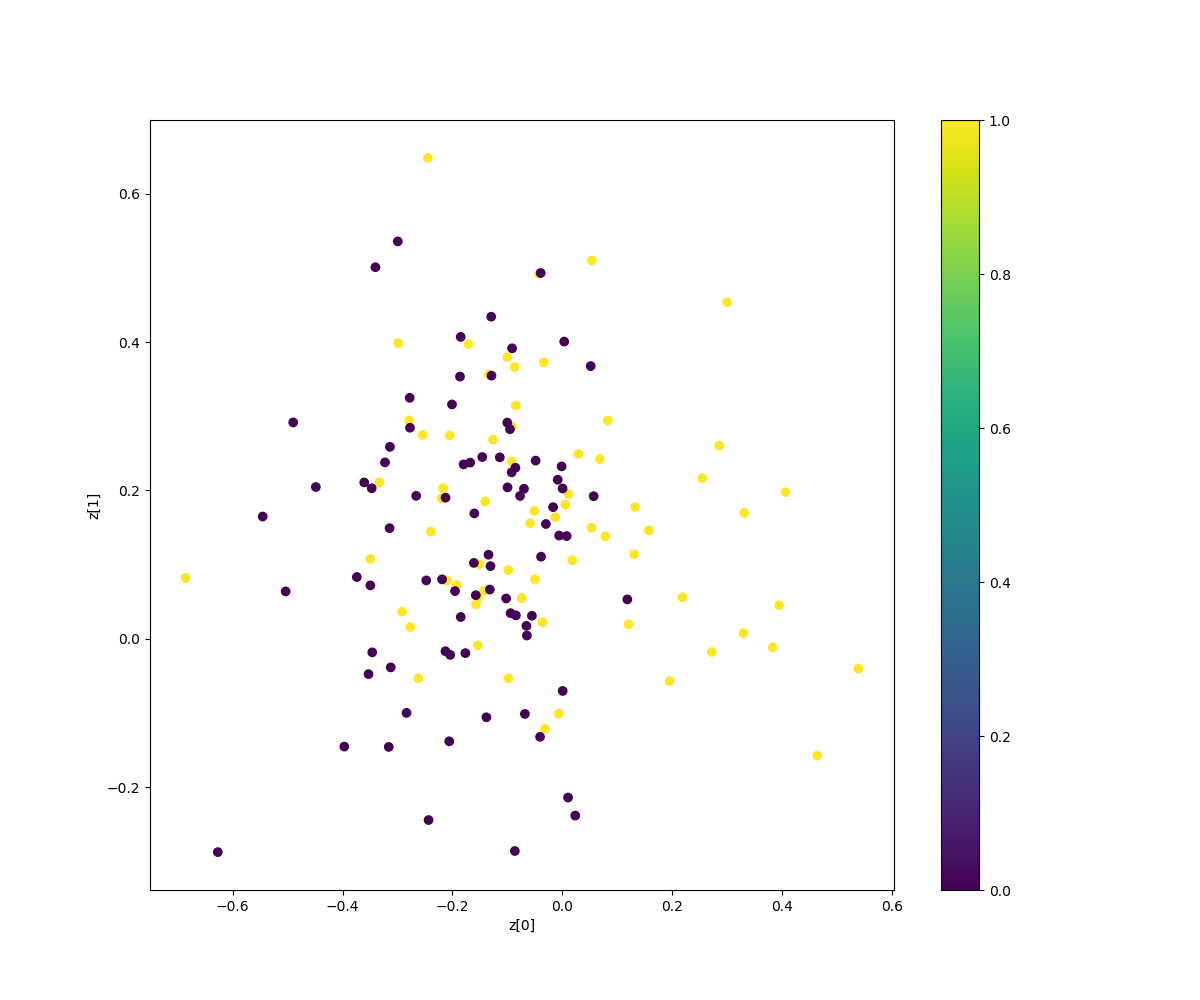
\includegraphics[clip, width=\linewidth]{fig/variational_auto_encoder/vae_colon_epoch_100_c13_he}
		\subcaption{HE like color at sample A}
		\label{fig:}
	\end{minipage}
	\begin{minipage}[b]{0.45\columnwidth}
		\centering
		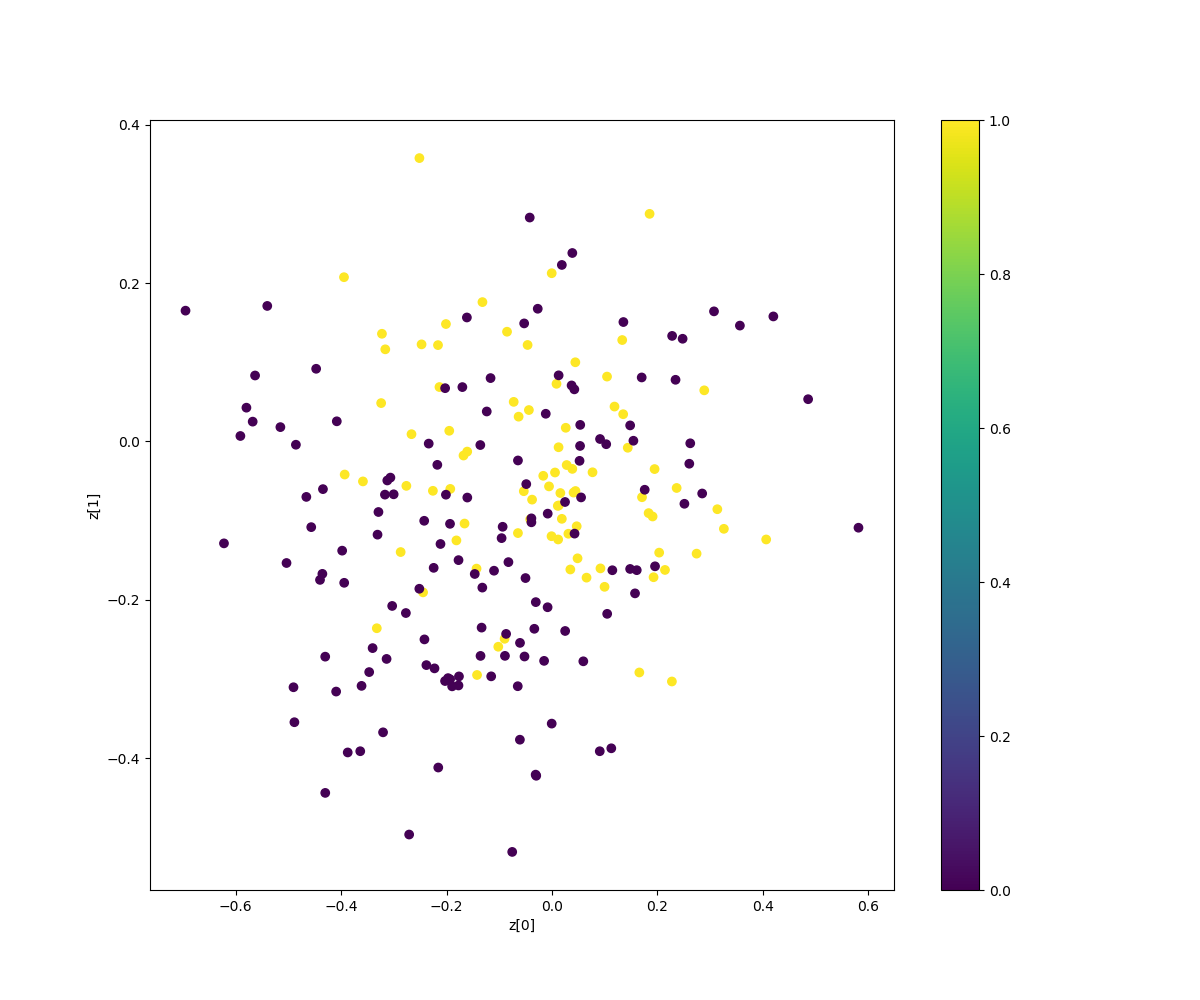
\includegraphics[clip, width=\linewidth]{fig/variational_auto_encoder/vae_colon_epoch_299_c13_rgb}
		\subcaption{original color at sample A}
		\label{fig:}
	\end{minipage}
	\begin{minipage}[b]{0.45\columnwidth}
		\centering
		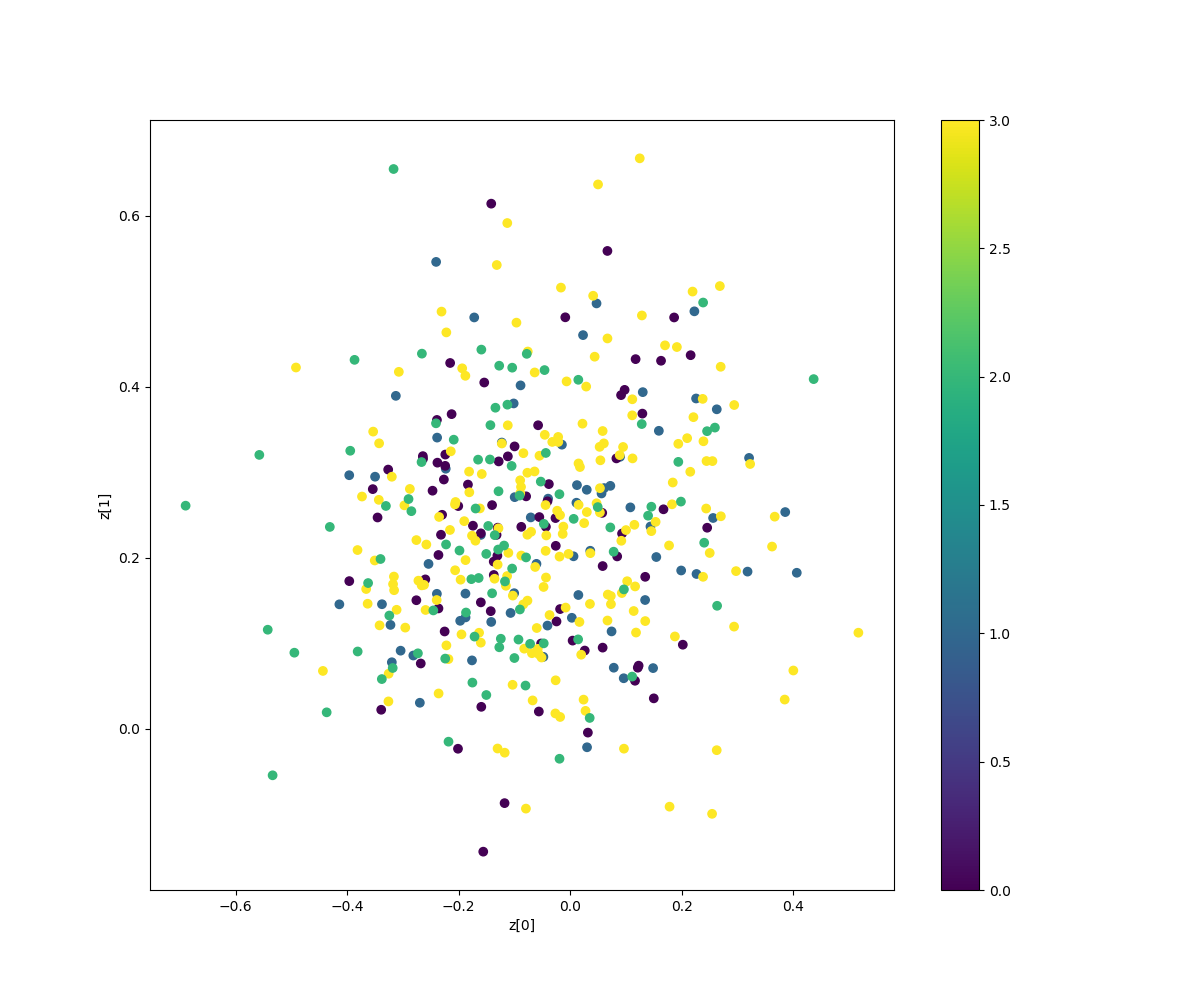
\includegraphics[clip, width=\linewidth]{fig/variational_auto_encoder/vae_colon_epoch_100_he_mix}
		\subcaption{HE like color at sample A and B}
		\label{fig:}
	\end{minipage}
	\begin{minipage}[b]{0.45\columnwidth}
		\centering
		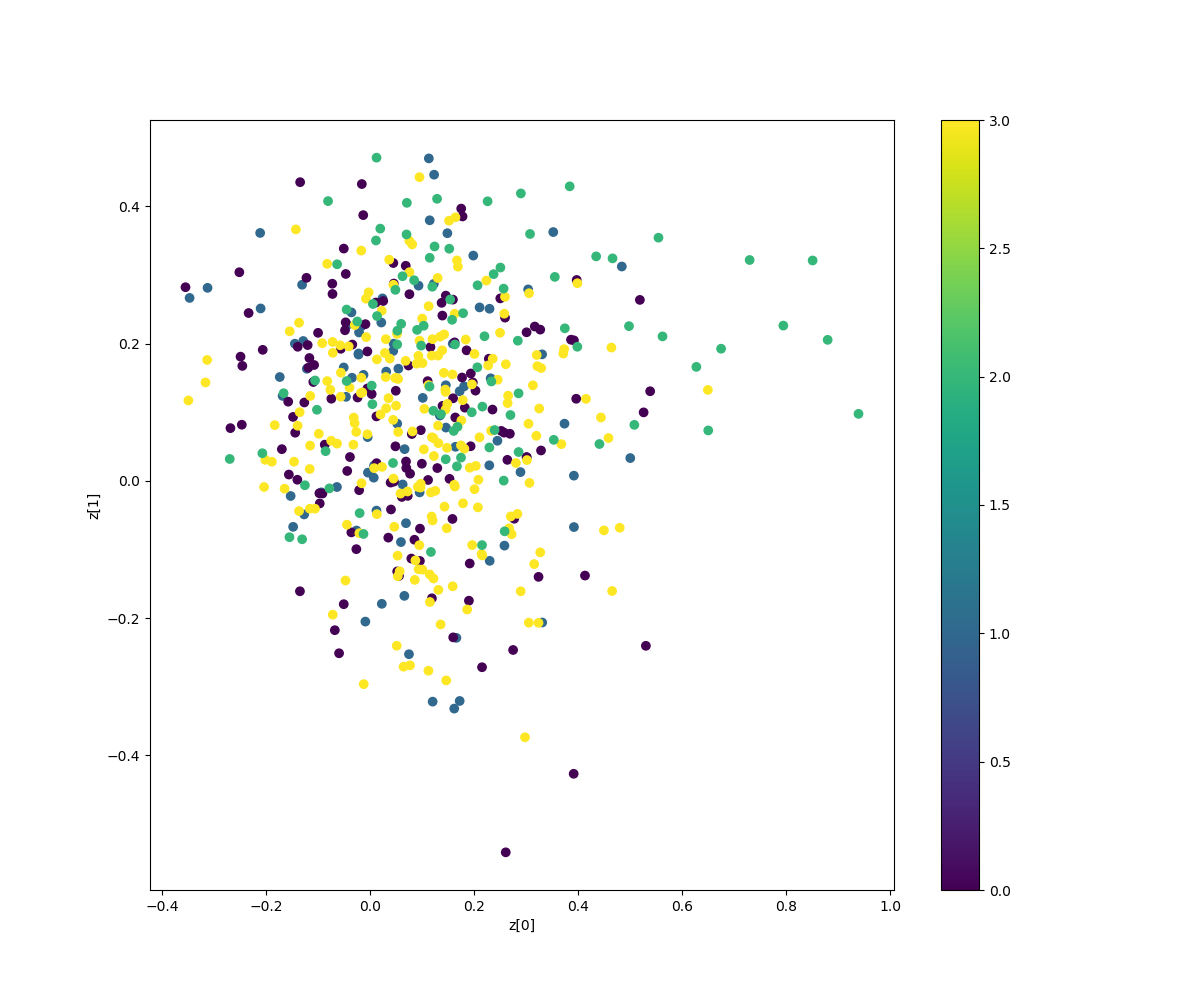
\includegraphics[clip, width=\linewidth]{fig/variational_auto_encoder/vae_colon_epoch_100_rgb_mix}
		\subcaption{original color at sample A and B}
		\label{fig:}
	\end{minipage}
	
	\caption{Latent space of 2D. Color ratio 1 is cancer, 0 is normal.}
	\label{fig:VAEplot}
	
\end{figure}

\subsection{GAN}

\begin{figure}[H]
	\centering
	
	\begin{minipage}{0.24\columnwidth}
		\centering
		
\includegraphics[clip, width=\linewidth]{fig/generative_adversarial_nets/0000_0000}
		\subcaption{epochs = 0}
		\label{fig:}
	\end{minipage}
	\begin{minipage}{0.24\columnwidth}
		\centering
		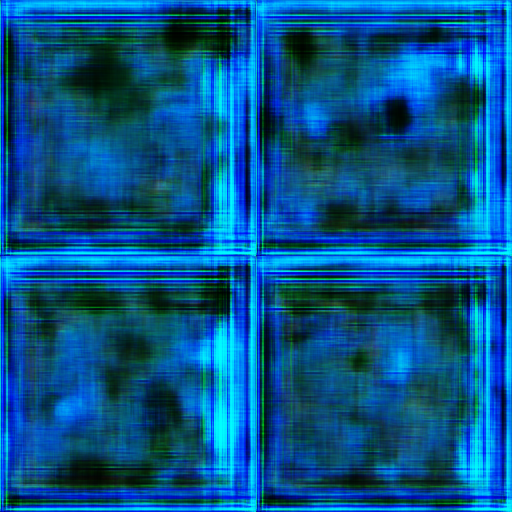
\includegraphics[clip, width=\linewidth]{fig/generative_adversarial_nets/0079_0000}
		\subcaption{epochs = 79}
		\label{fig:}
	\end{minipage}
	\begin{minipage}{0.24\columnwidth}
		\centering
		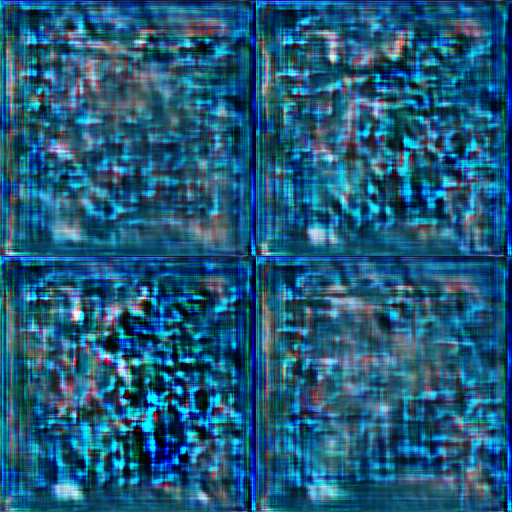
\includegraphics[clip, width=\linewidth]{fig/generative_adversarial_nets/0641_0000}
		\subcaption{epochs = 641}
		\label{fig:}
	\end{minipage}
	\begin{minipage}{0.24\columnwidth}
		\centering
		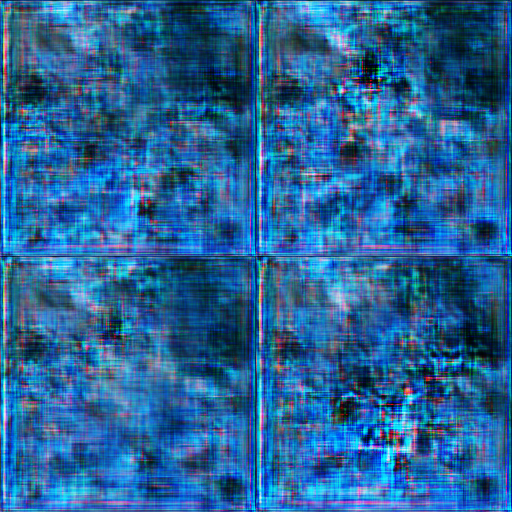
\includegraphics[clip, width=\linewidth]{fig/generative_adversarial_nets/0969_0000}
		\subcaption{epochs = 969}
		\label{fig:}
	\end{minipage}
	\begin{minipage}{0.24\columnwidth}
		\centering
		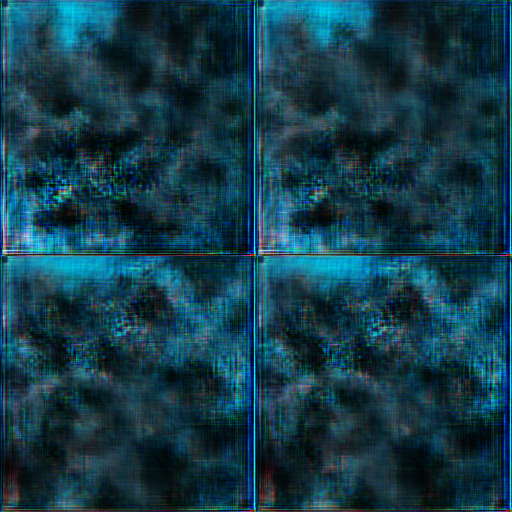
\includegraphics[clip, width=\linewidth]{fig/generative_adversarial_nets/1213_0000}
		\subcaption{epochs = 1213}
		\label{fig:}
	\end{minipage}
	\begin{minipage}{0.24\columnwidth}
		\centering
		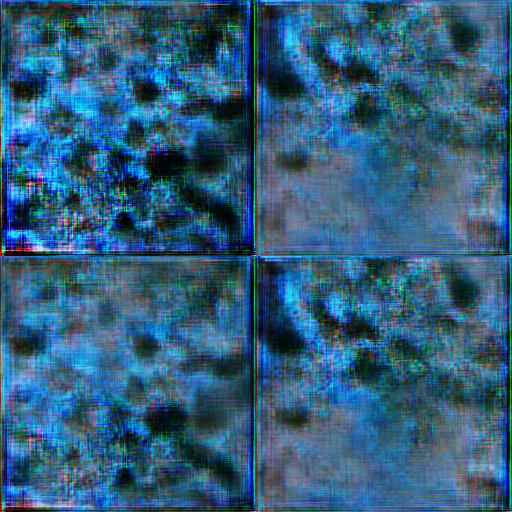
\includegraphics[clip, width=\linewidth]{fig/generative_adversarial_nets/1619_0000}
		\subcaption{epochs = 1619}
		\label{fig:}
	\end{minipage}
	\begin{minipage}{0.24\columnwidth}
		\centering
		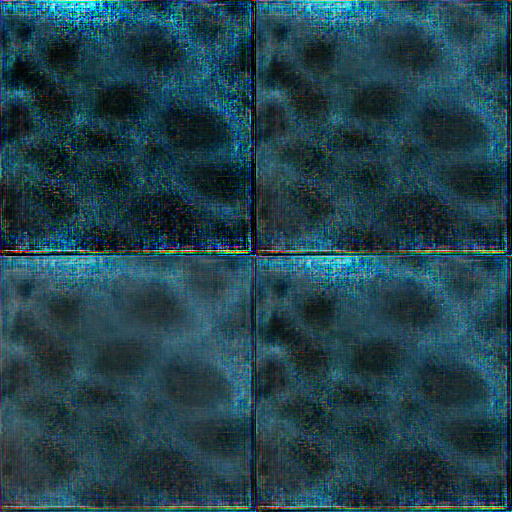
\includegraphics[clip, width=\linewidth]{fig/generative_adversarial_nets/2004_0000}
		\subcaption{epochs = 2004}
		\label{fig:}
	\end{minipage}
	\begin{minipage}{0.24\columnwidth}
		\centering
		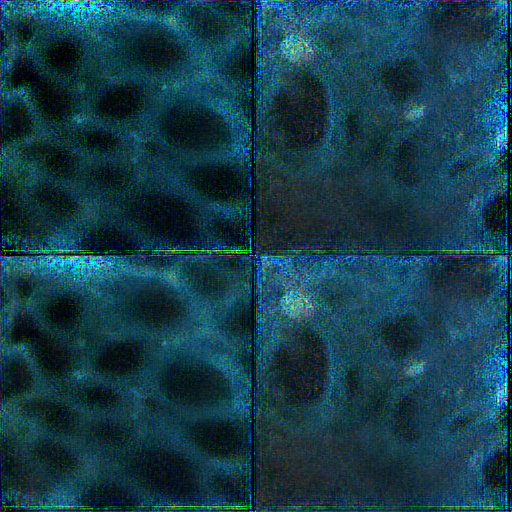
\includegraphics[clip, width=\linewidth]{fig/generative_adversarial_nets/3208_0000}
		\subcaption{epochs = 3208}
		\label{fig:}
	\end{minipage}
	
	\caption{Transition generated images by GAN}
	\label{fig:GANimage}
	
\end{figure}


\section{半教師あり学習による識別精度評価}

%lossとaccグラフ
% 教師ありと半教師ありを同じグラフにaccをプロット